\documentclass[class=report, crop=false, 12pt,a4paper]{standalone}
\usepackage{enumitem}
\usepackage{tikz}
\usepackage{float}
\usepackage{graphicx}
\usepackage{multicol}
\usepackage{siunitx}
\usepackage{mathtools}
\usepackage{amsmath}
\usepackage{amssymb}
\usepackage{commath}
\usepackage[normalem]{ulem}
\usepackage[a4paper,width=150mm,top=25mm,bottom=25mm]{geometry}
\begin{document}
\begin{center}
  30/11/2020
\end{center}
There are many ways to measure temperature, including changes of:
\begin{enumerate}
  \item Pressure/volume (thermal expansion) – generic thermometer;
  \item Contact potential between different metals – thermocouple;
  \item Resistance of a metal or a semiconductor – thermistor;
  \item Energy radiated by a hot object – radiation pyrometer.
\end{enumerate}
\begin{figure}[H]
  \centering
  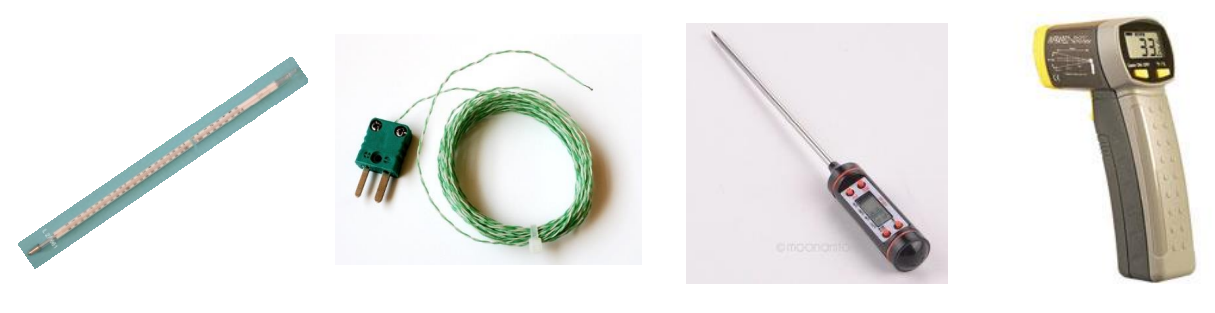
\includegraphics[width = 0.8\textwidth]{../img/Mdiagram57.png}
\end{figure}
Note: None of the properties of materials used for temperature sensing varies strictly linearly with temperature. Thus, calibration is very important for temperature transducers.
\section{Standard Temperature for Calibration}
In the IPTS (the International Practical Temperature Scale), values of temperature are assigned to the eleven reproducible fixed points shown below.
\begin{figure}[H]
  \centering
  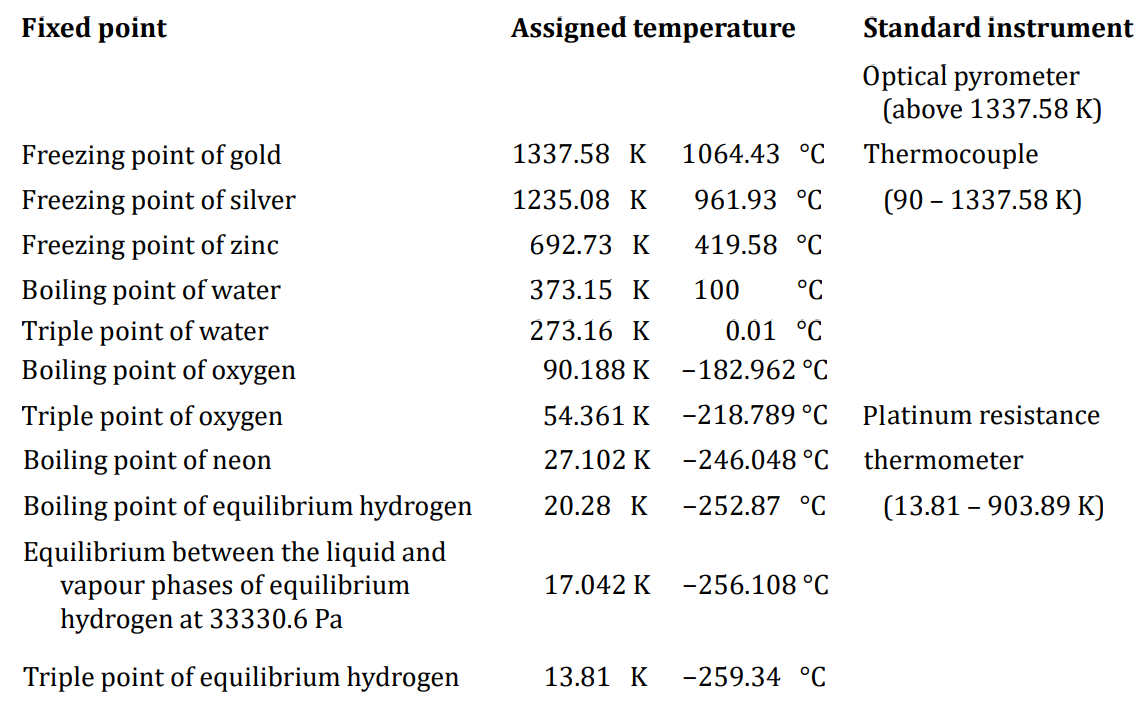
\includegraphics[width = 0.9\textwidth]{../img/Mdiagram59.png}
\end{figure}
\section{Measurement Using Changes in Volume/Pressure}
Thermal expansion is the key.
\begin{figure}[H]
  \centering
  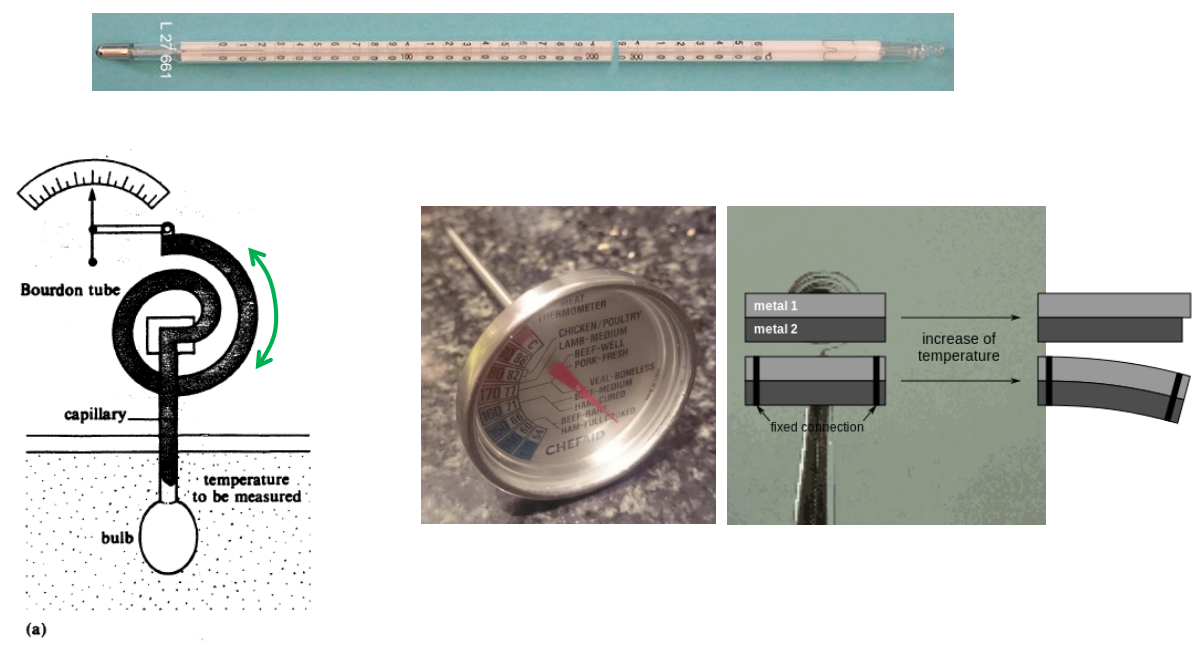
\includegraphics[width = 0.8\textwidth]{../img/Mdiagram60.png}
\end{figure}
\section{Thermoelectric Temperature Sensors (Thermocouples)}
A thermocouple consists of two wires of different metals joined at both ends. If the junctions between the metals are at different temperatures, an electric current will flow around the circuit. This phenomenon is called \textbf{thermoelectric or Seebeck effect}.
\begin{figure}[H]
  \centering
  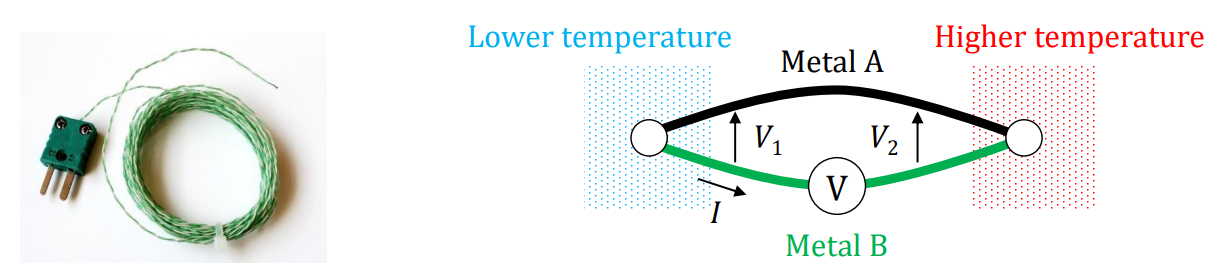
\includegraphics[width = 1\textwidth]{../img/Mdiagram61.png}
\end{figure}
Across the junction of any two dissimilar metals, there always appear a difference in electric potential called the ‘contact potential’. The contact potential varies with the temperature at the junction between the two metals, increasing in magnitude with an increase in temperature.
\subsection{Thermocouples in practice}
Contact potential could also occur at the junction between metal B and the wires leading to the voltmeter, unless the wire is made of metal B (very unlikely), generating contact potential $V_3$ and $V_4$.
\begin{figure}[H]
  \centering
  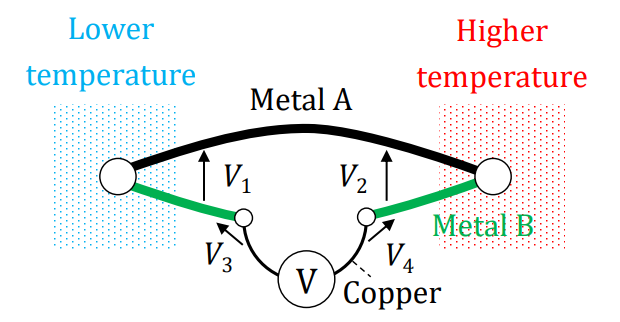
\includegraphics[width = 0.6\textwidth]{../img/Mdiagram62.png}
\end{figure}
In practice, it does not matter as long as the junctions are kept under the same temperature (i.e. $V_3 = V_4$).
\begin{figure}[H]
  \centering
  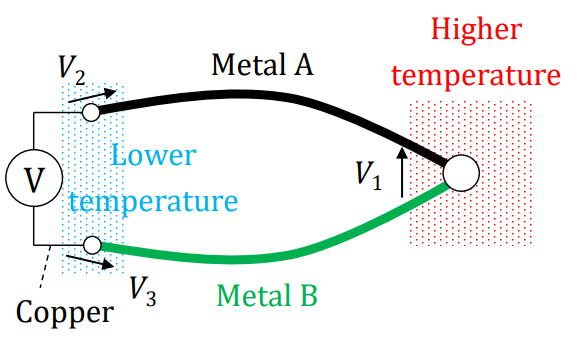
\includegraphics[width = 0.6\textwidth]{../img/Mdiagram63.png}
\end{figure}
An alternative configuration is the one in the bottom panel. Here, the net contact potential is $V_1+V_3-V_2$.
\subsection{Thermocouple materials and construction}
Various standards have been developed for thermocouples, with the relevant British Standard being BS4937, part of which is shown below.
\begin{figure}[H]
  \centering
  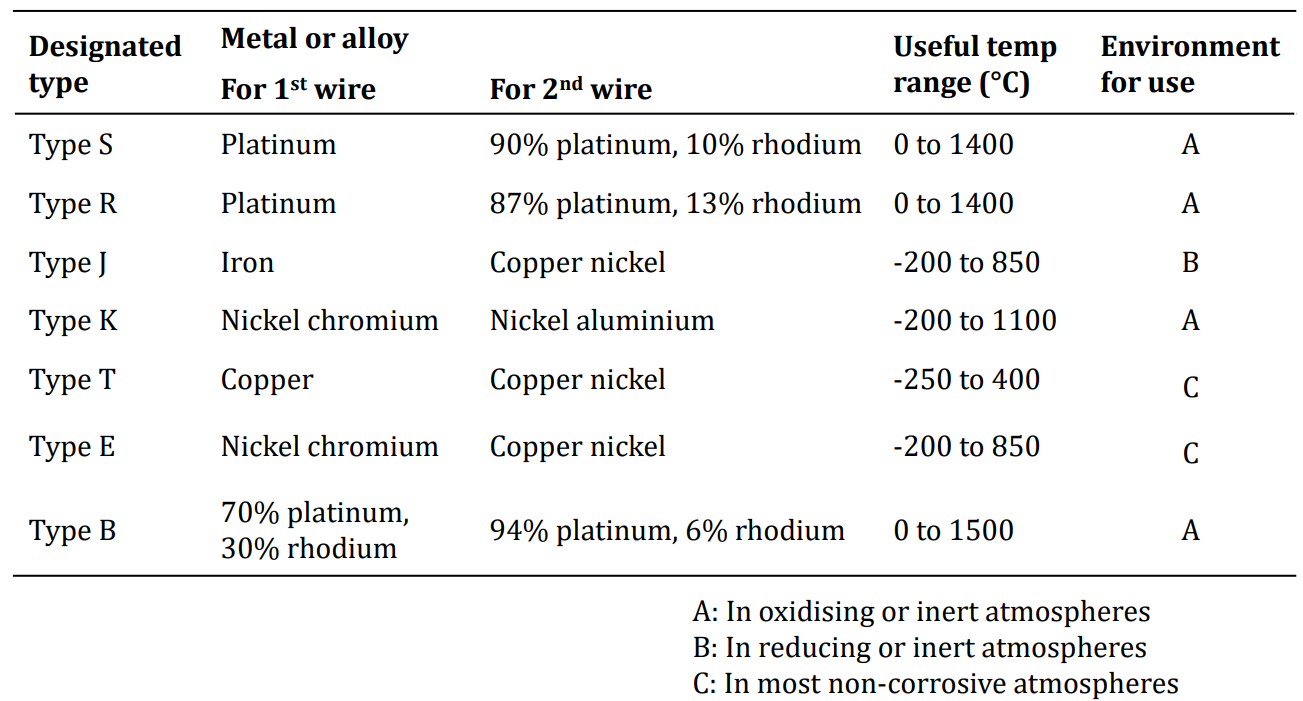
\includegraphics[width = 0.9\textwidth]{../img/Mdiagram64.png}
\end{figure}
The choice of the right thermocouple for any application depends on:
\begin{itemize}
  \item The sensitivity as well as the temperature range (shown in the figure)
  \item Applicability in corrosive environments
  \item Whether it can withstand thermal and mechanical stresses
  \item Accuracy and reproducibility
  \item Price
\end{itemize}
\begin{figure}[H]
  \centering
  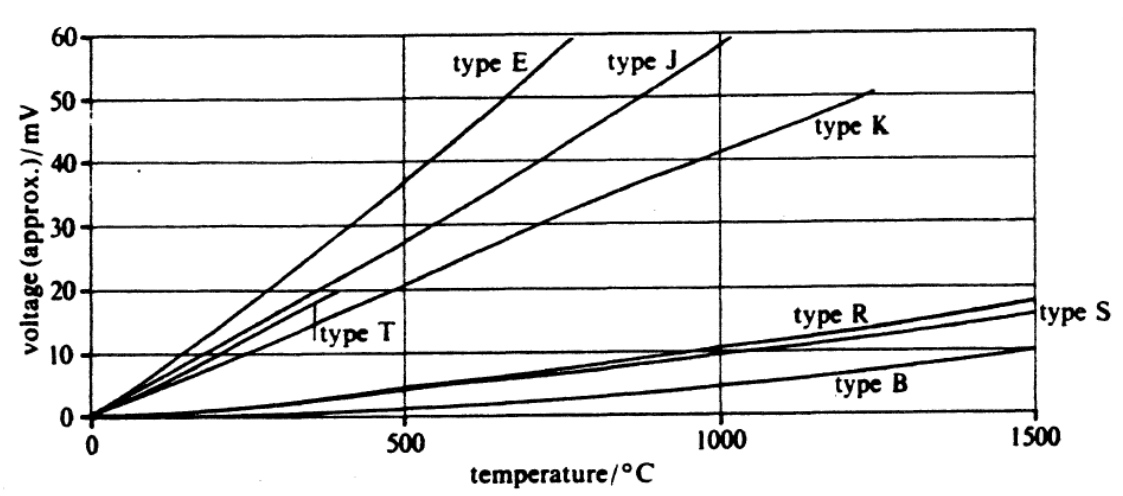
\includegraphics[width = 0.9\textwidth]{../img/Mdiagram65.png}
\end{figure}
\subsection{Thermocouple structure}
Thermocouples can have 2 different types of probe ends:
\begin{enumerate}
  \item Soldered bare wire
  \item With metallic sheath
\end{enumerate}
\begin{figure}[H]
  \centering
  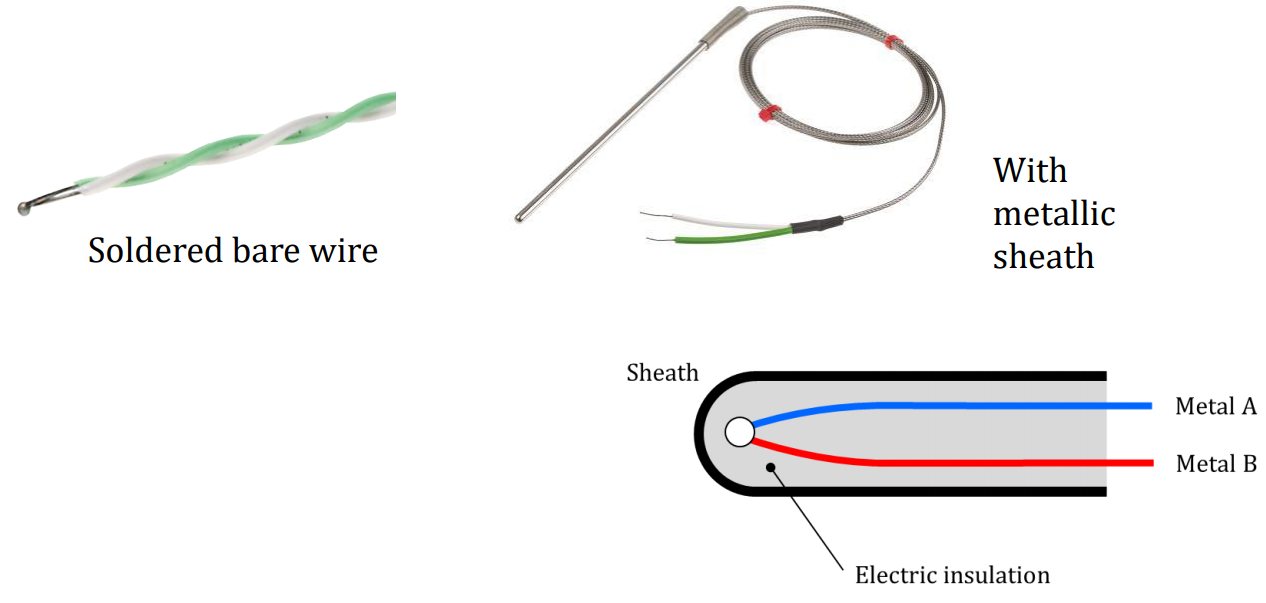
\includegraphics[width = 0.8\textwidth]{../img/Mdiagram66.png}
\end{figure}
The main differences between the two different types:
\begin{itemize}
  \item With a metallic sheath, the probe can touch conductive surfaces
  \begin{itemize}
    \item Sheath has electric insulation inside, so the reading won't be affected
  \end{itemize}
  \item Longer response time
  \begin{itemize}
    \item The metallic sheath and the electric insulation must be heated up first before reaching the joint inside
  \end{itemize}
  \item Insulation material needs to be high electric resistance + high thermal conductivity
\end{itemize}
\section{Basic Metallic Resistance Thermometers}
\begin{figure}[H]
  \centering
  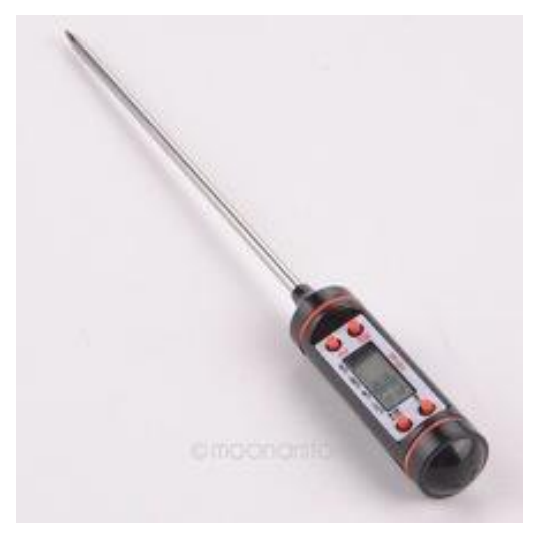
\includegraphics[width = 0.25\textwidth]{../img/Mdiagram68.png}
\end{figure}
The resistance of certain metals varies with temperature. The resistance $R_T$ at temperature $T$ is approximately shown relative to the resistance $R_0$ at $\ang{0}$C, using the following equation: 
\begin{gather}
  R_T = R_0 (1+\alpha T)
\end{gather}
Where:
\begin{itemize}
  \item $\alpha$ is called the temperature coefficient of resistance
\end{itemize}
This could be described more generally:
\begin{gather}
  R_T = R_0(1+\alpha(T-T_0))
\end{gather}
taking $T_0$ as the reference temperature fro $R_0$.
\begin{figure}[H]
  \centering
  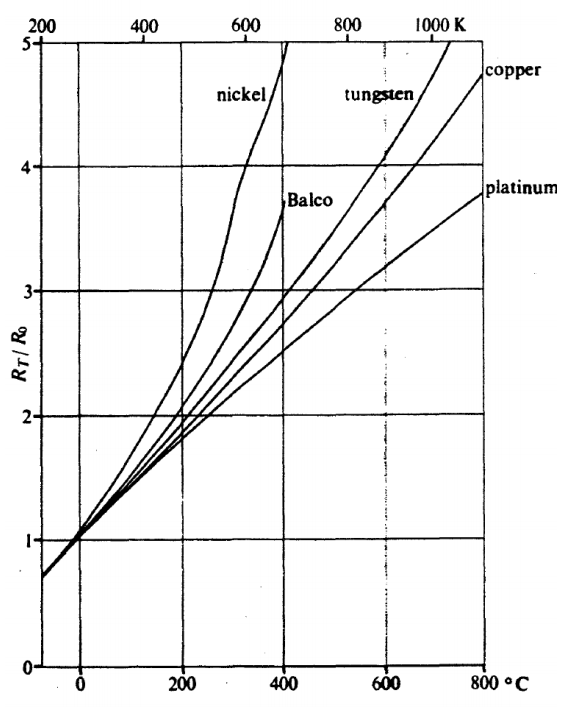
\includegraphics[width = 0.6\textwidth]{../img/Mdiagram67.png}
\end{figure}
The figure shows the relative resistance variation of certain metals over temperature (using $R_0$ at $\ang{0}$C). Although the sensitivity of platinum is the smallest, it has advantage of:
\begin{itemize}
  \item Most stable and reproducible (linear),
  \item Chemically inert and resistant to contamination.
\end{itemize}
Typical resistance thermometer construction includes:
\begin{itemize}
  \item A type with its platinum coil of wire directly exposed to the fluid whose temperature is to be measured.
  \item The resistance wire is isolated from the fluid, so that the resistance wire does not become contaminated with other materials which could change the relationship of its resistance to temperature. The ceramic rod is to help the sensor to withstand mechanical shock.
  \item The resistance metal is deposited as a thin film pattern on an insulating substrate. This type of sensor can be attached to a flat surface.
\end{itemize}
\begin{figure}[H]
  \centering
  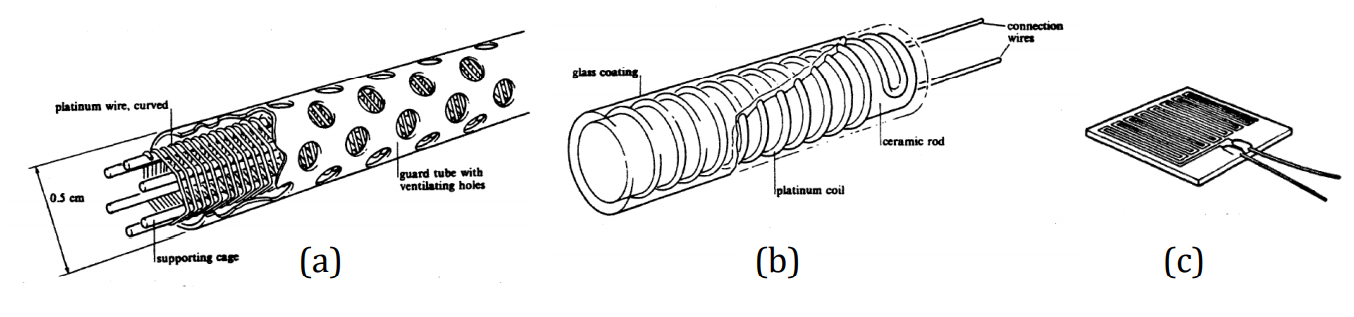
\includegraphics[width = 1\textwidth]{../img/Mdiagram69.png}
\end{figure}
Errors can be caused by:
\begin{itemize}
  \item Self-heating effect – electric current flows through the resistance wire heats the resistor up because of energy dissipation.
  \item Thermoelectric effect – likewise thermocouple, if the resistance wire and the lead wire are made of different metal, an additional electric current will flow due to thermoelectric effect.
\end{itemize}
\section{Thermistors}
THERM-ally sensitive res-ISTOR
\begin{figure}[H]
  \centering
  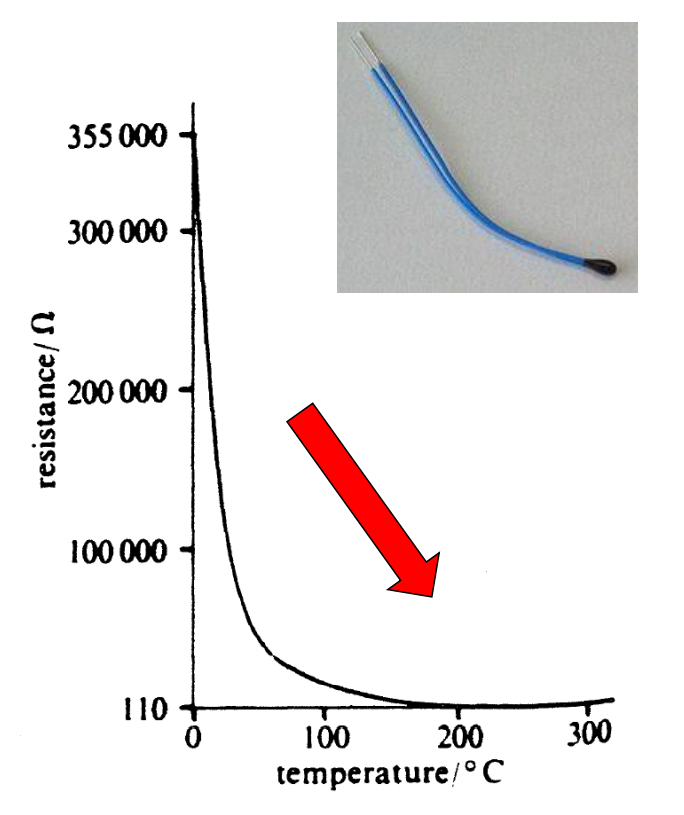
\includegraphics[width = 0.6\textwidth]{../img/Mdiagram70.png}
\end{figure}
The resistance against temperature curve for a thermistor (semiconductor) is very different from that for metallic resistance thermometers. It decreases with temperature rather than increase, and the negative temperature coefficient of resistance in this case is much larger than that of metals. \\\\
The relationship between $R_T$ and temperature $T$ for thermistor can be modelled as:
\begin{gather}
  R_T = A\cdot e^{\frac{B}{T}}
\end{gather}
Where:
\begin{itemize}
  \item A and B are constants. 
  \item B is called the characteristic temperature of the thermistor (material constant) whose value is normally between 2000 K and 4000 K.
\end{itemize}
If the resistance at a temperature $T_0$ is known (for example, base resistance at room temperature),
\begin{gather}
  R_0 = A\cdot e^{\frac{B}{T_0}}
\end{gather}
and combining the two equation:
\begin{gather}
  R_T = R_0\exp\left(B\left[\frac{1}{T}-\frac{1}{T_0}\right]\right)
\end{gather}
Thermistors can be made \textbf{much smaller} than metallic resistance thermometers. This enables them to \textbf{respond to temperature variation more quickly}. However, this also means that the \textbf{self-heating effect is greater} for the same current than metallic sensors, and so they must be operated at smaller current levels.
\subsection{Measuring circuits for resistive sensors}
\begin{figure}[H]
  \centering
  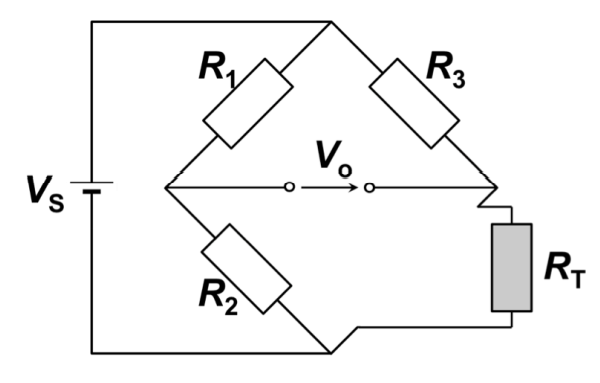
\includegraphics[width = 0.5\textwidth]{../img/Mdiagram71.png}
\end{figure}
We use Wheatstone bridge for resistive sensors and the output voltage from the bridge is:
\begin{gather}
  V_o = \left(\frac{R(1+x)}{R(1+x)+R}-\frac{1}{2}\right)V_S = \frac{x}{2(2+x)}V_S
\end{gather}
Where $x$ is increase in the resistance due to the measurement and all resistors are assumed to have the same resistance at reference temperature. \textbf{If $x$ is small enough}, this can be approximated as:
\begin{gather}
  V_o = \frac{x}{4}V_S
\end{gather}
But this does not apply to resistive temperature sensors, that is thermistors ($x$ is large) and the bridge output voltage becomes highly nonlinear against $T$. \\\\
A simple workaround is not to measure $V_o$ but to vary $R_2$ (by use of potentiometer) such that the bridge is balanced. If $R_1 = R_3$, $R_2 = R_T$ allows calculation of $T$, based on the following relationships. \\\\
Resistance thermometer:
\begin{gather}
  R_T = R_0(1+\alpha(T-T_0))
\end{gather}
Thermocouple:
\begin{gather}
  R_T = R_0\exp\left(B\left[\frac{1}{T}-\frac{1}{T_0}\right]\right)
\end{gather}
\section{Pyrometer and Radiation}
Radiation pyrometers detect the infrared radiation given off by the object whose temperature is being measured. Radiation pyrometers can be used to measure temperatures as low as $\ang{-50}$C, so infrared radiation is not only emitted by hot bodies. Any object whose temperature is not at absolute zero (0 K) emits radiation. \\\\
Radiation = travel of energy wave (like X-ray)
\begin{itemize}
  \item Does not require medium to propagate
  \item $\neq$ sound (which requires medium to travel)
\end{itemize}
\subsection{Black body}
A body at a certain temperature emits a certain amount of energy with a certain spectrum (see figure below). Note: An ideal body, blackbody, emits radiation in all wavelengths. This is used to measure temperature in approximate manner.
\begin{figure}[H]
  \centering
  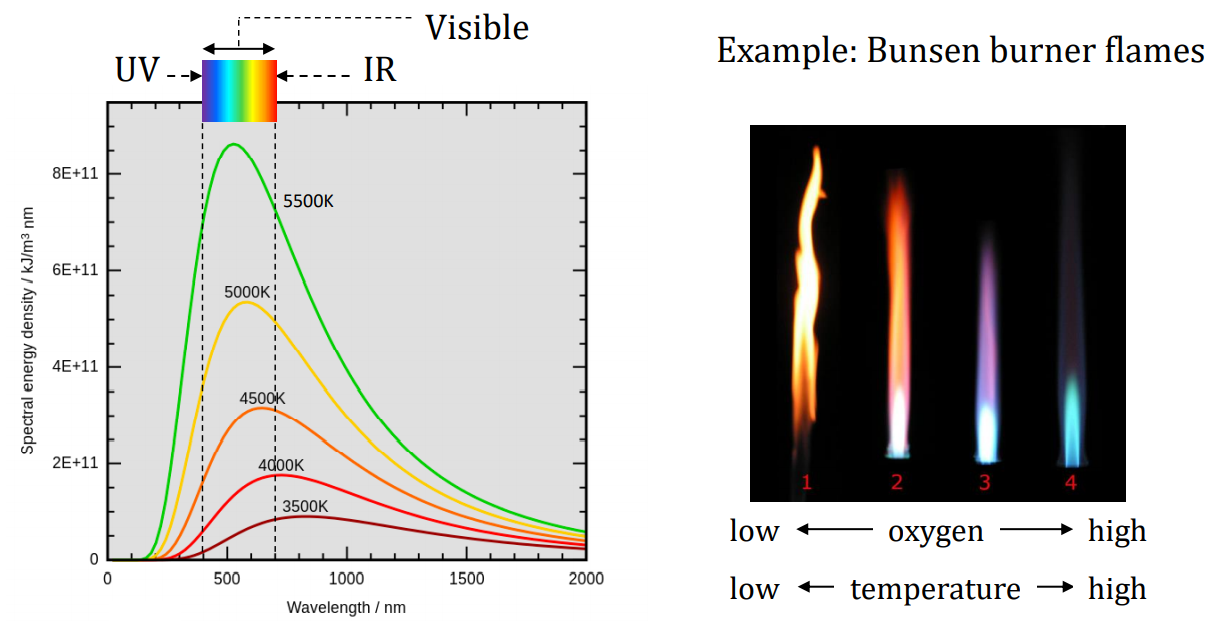
\includegraphics[width = 0.9\textwidth]{../img/Mdiagram72.png}
\end{figure}
\subsection{Radiation pyrometers}
\begin{figure}[H]
  \centering
  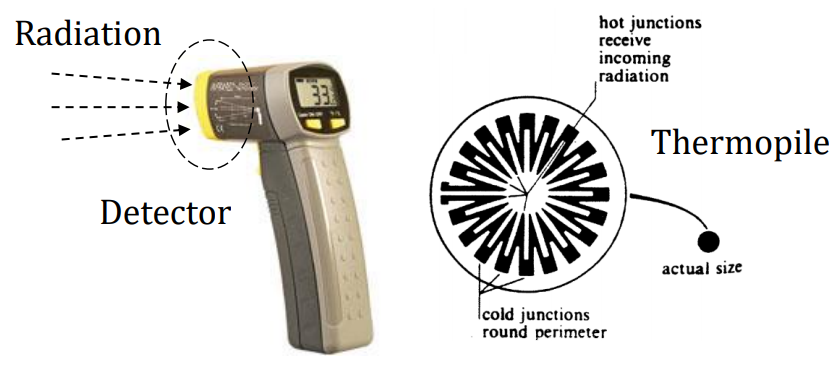
\includegraphics[width = 0.75\textwidth]{../img/Mdiagram73.png}
\end{figure}
\subsubsection{Working principle:}
Temperature transducer is used in the detector (e.g. thermopile), the detected temperature is converted to the radiation energy using Stefan-Boltzmann law.
\begin{gather}
  M = \sigma T_{detected}^4
\end{gather}
\begin{itemize}
  \item Note: $T_{detected}$ is the  temperature due to radiation and not the temperature of the surface
\end{itemize}
The energy is then converted to temperature of the measured surface using the black body energy plot.
\subsubsection{Some features}
\begin{itemize}
  \item Very short response time
  \item Reflective or transparent/translucent surface is likely to lead to error
  \item Distance independent measurement
\end{itemize}
\begin{figure}[H]
  \centering
  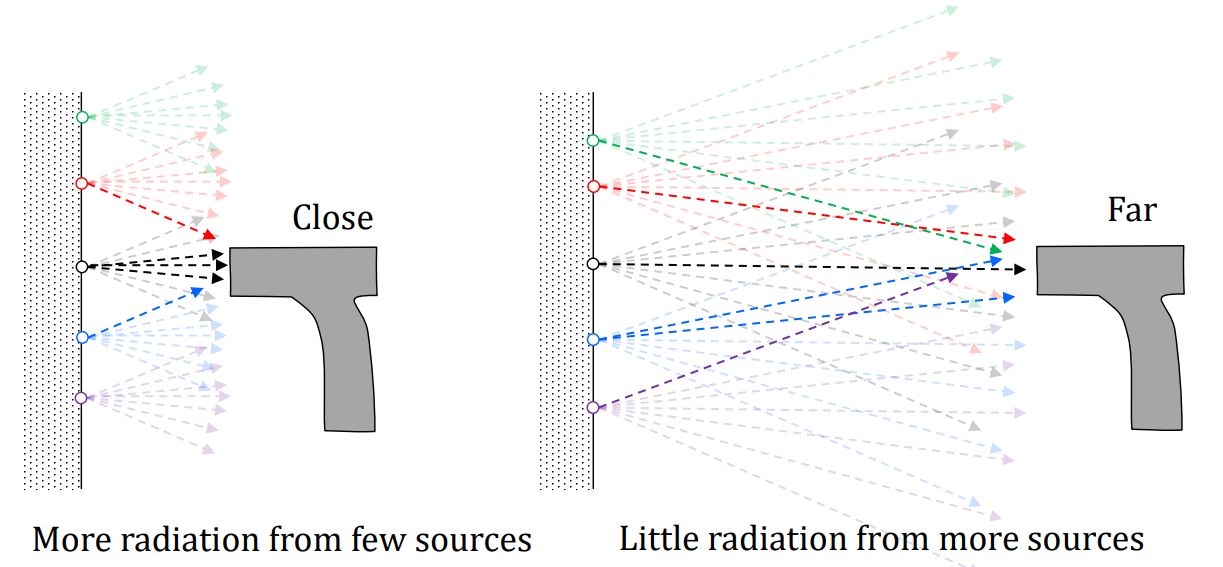
\includegraphics[width = 1\textwidth]{../img/Mdiagram74.png}
\end{figure}
\section{Temperature Response}
A challenge of temperature measurement $\longrightarrow$ \textbf{no thermometer can respond instantly to a change in temperature}. The response is expressed mathematically as:
\begin{gather}
  \frac{\dif T}{\dif t} \propto (T_f-T) \ \ \ \text{or} \ \ \ \frac{\dif T}{\dif t}+KT = KT_f
\end{gather}
Where:
\begin{itemize}
  \item $K$ is a constant 
  \item $T_f$ is the temperature to be measured
\end{itemize}
The general solution is: 
\begin{gather}
  T = A\cdot e^{-Kt}+T_f = (T_0-T_f)\cdot e^{-Kt} + T_f
\end{gather}
The speed of change is characterised by the time constant $\tau (=1/K)$ which is the time interval in which the temperature varies 63.2\% of the difference between initial and final temperatures.
\begin{figure}[H]
  \centering
  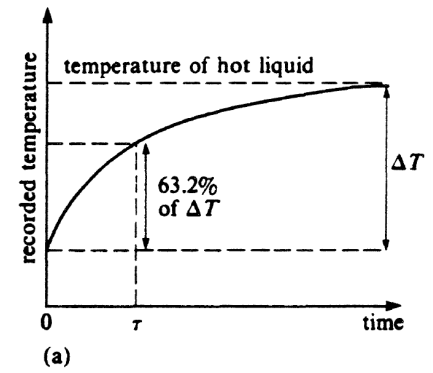
\includegraphics[width = 0.5\textwidth]{../img/Mdiagram75.png}
\end{figure}
\subsection{Transient temperature response}
If the transducer is subjected to a sinusoidally varying input temperature, the differential equation becomes:
\begin{gather}
  \frac{\dif T}{\dif t}+KT = KT_f = KT_a\sin(\omega t)
\end{gather}
The solution of this equation in terms of the time-constant $\tau$ is:
\begin{gather}
  y = A\cdot e^{\frac{-t}{\tau}}+\frac{T_a}{\sqrt{1+\omega^2\tau^2}}\sin(\omega t+\varphi)
\end{gather}
Where:
\begin{itemize}
  \item $\varphi = \tan^{-1}(\omega/k)$. The figure below shows the two temperature variations.
\end{itemize}
\begin{figure}[H]
  \centering
  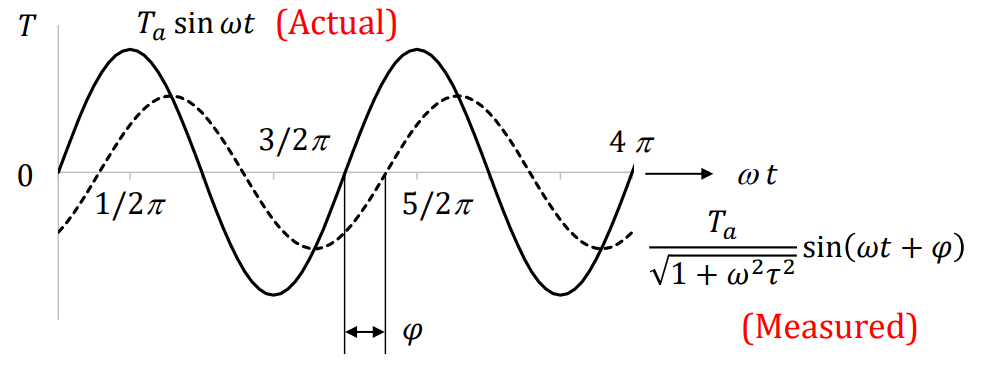
\includegraphics[width = 0.9\textwidth]{../img/Mdiagram76.png}
\end{figure}
\end{document}